%%%%%%%%%%%%%%%%%%%%%%%%%%%%%%%%%%%%%%%%%%%%%%%%%%%%%%%%%%%%%%%%%%%%%%%%%%%%%%%%
\chapter{Conclusion and Future Work}\label{ch:conclusion}
%%%%%%%%%%%%%%%%%%%%%%%%%%%%%%%%%%%%%%%%%%%%%%%%%%%%%%%%%%%%%%%%%%%%%%%%%%%%%%%%


\section{Future Work}

With the work done so far and the results achieved, we may identify the current limitation of our project, and plan improvements to solve these issues. 
We can list as  main weak points right now:

\begin{itemize}
	\item Poor performance of the Trace Analyzer and Sniffer components;
	\item Weak scaling results of the traffic generator using \textit{libtins}.
\end{itemize}

And as further implementations, but with low priority, we may have:

\begin{itemize}
	\item Support for new traffic generator tools;
	\item APIs for the Flow Generator on  Python and Lua, wich have cosolidate traffic generator APIs;
	\item A \textit{pcap-crafter} component. Instead of creating traffic, creates a \textit{pcap} file.
\end{itemize}

Identified these issues and possible future works, we conceived approaches and methods to achieve these results. They include improvements on the implementation,  calibration of constants\footnote{Calibration here means to test many values, and see which one can improve our outcomes for a large variety of traces of traces.}, a finner control of packet injection, use of new technologies and newer implementations. As we always did in the project, we create a task list of activities and organize them by priority and goal. They are listed in the table ~\ref{tab:task-list}.  


\begin{table}[ht!]
	\centering
	\caption{Future Work: task list}
	\label{tab:task-list}
	\begin{tabular}{cccc}
		\hline
		\multicolumn{3}{c}{Future Work}	& Priority \\ \hline
		1                      & Optimizing linear regression                              &                                                 & \textit{high}                    \\
		2                      & Flow-merging option                                       &                                                 & medium                  \\
		3                      & Smart flow-scheduler                                      &                                                 & \textit{high}                    \\
		4                      & \texttt{DataProcessor::minimumAmountOfPackets}                         &                                                 & low                     \\
		5                      & DPDK KNI interfaces                                       &                                                 & medium                     \\
		6                      & Multi-thread C++ sniffer                                  & \multirow{-6}{*}{Performance}                   & \textit{high}                    \\ \hline
		7                      & Model inter-packet times on \texttt{TinsFlow}           &                                                 & \textit{high}                    \\
		8                      & D-ITG flow generator (\texttt{DitgFlow})                &                                                 & low                     \\
		9                      & DPDK flow generator (\texttt{DpdkFlow})                 &                                                 & medium                     \\
		10                     & Ostinato flow generator (\texttt{OstinatoFlow})         & \multirow{-4}{*}{Tool support}                  & low                     \\ \hline
		11                     & \texttt{DataProcessor::min\_time}                       &                                                 & low                     \\
		12                     & \texttt{DataProcessor::m\_min\_on\_time}                &                                                 & low                     \\
		13                     & \texttt{DataProcessor::m\_session\_cut\_time}           &                                                 & low                     \\
		14                     & Minimum number of packets per flow option                 & \multirow{-4}{*}{Calibration}  & low                     \\ \hline
		15 & Python API/Lua for traffic generation & & low \\
		16 & Crafter of  pcap files & \multirow{-2}{*}{New features} & low \\
		%17 & Json compact trace descriptor  & \multirow{-3}{*}{New features} & low 
		\hline
	\end{tabular}
\end{table}



(1) The major issue of SIMITAR now is optimizing data processing for creating the compact trace descriptor. The performance becomes an issue when processing large \textit{pcap} files with more dozens of thousands of flows. The time expended for processing traces, in this case, is exceeding tens of hours. In the current implementation, the linear regression execution is mono-thread, and the stop criterion is just the number of iterations. Parallel processing, and creating stop criteria based on convergence in addition to the number of iterations will improve the performance. 

(2) Crating an option for merging flows is a possibility to improve the performance of traffic with several thousands of flows and Gigabits of bandwidth, such as from WAN captures. A merge criterion, for example, is to consider just network headers on flow's classification.


(3) Currently, all the flow threads are instantiated once the traffic generations start. A smarter traffic generation where SIMITAR instantiates each thread when the traffic, and join when it is inactive should reduce the overhead for traces with a large number of flows. For traffics with a massive amount of streams, a methodology for merging them should reduce computational costs and enable replication of traffic with a much more significant bandwidth. 


(4) Constant \texttt{DataProcessor::minimumAmountOfPackets}: SIMITAR only estimates stochastic models for inter-packet times if the number of packets for this flow is larger than this amount. If it is smaller, SIMITAR just uses the constant model. We decide to do it for two reasons. First, because with a small sample, the modeling accuracy is poor . Second, we avoid the cost of the parameterization process. Now, its value is set to Its value today is set to 30. Increasing this amount, we may achieve a more reasonable performance for individual flows, and reduce the processing time. 


(5) One possibility to improve the traffic generation performance issue DPDK Kernel NIC Interface  (KNI interfaces) \footnote{\href{http://dpdk.org/doc/guides/prog_guide/kernel_nic_interface.html}{http://dpdk.org/doc/guides/prog\_guide/kernel\_nic\_interface.html}}. DPDK KNI interfaces allow applications from the user's space interact with DPDK ports. In this way, we may achieve a faster packet processing. This can be integrated as an insatiable feature of SIMITAR (figure ~\ref{fig:dpdk-if}).


\begin{figure}[h!]
	\centering
	\subfloat[DpdkFlow]{
		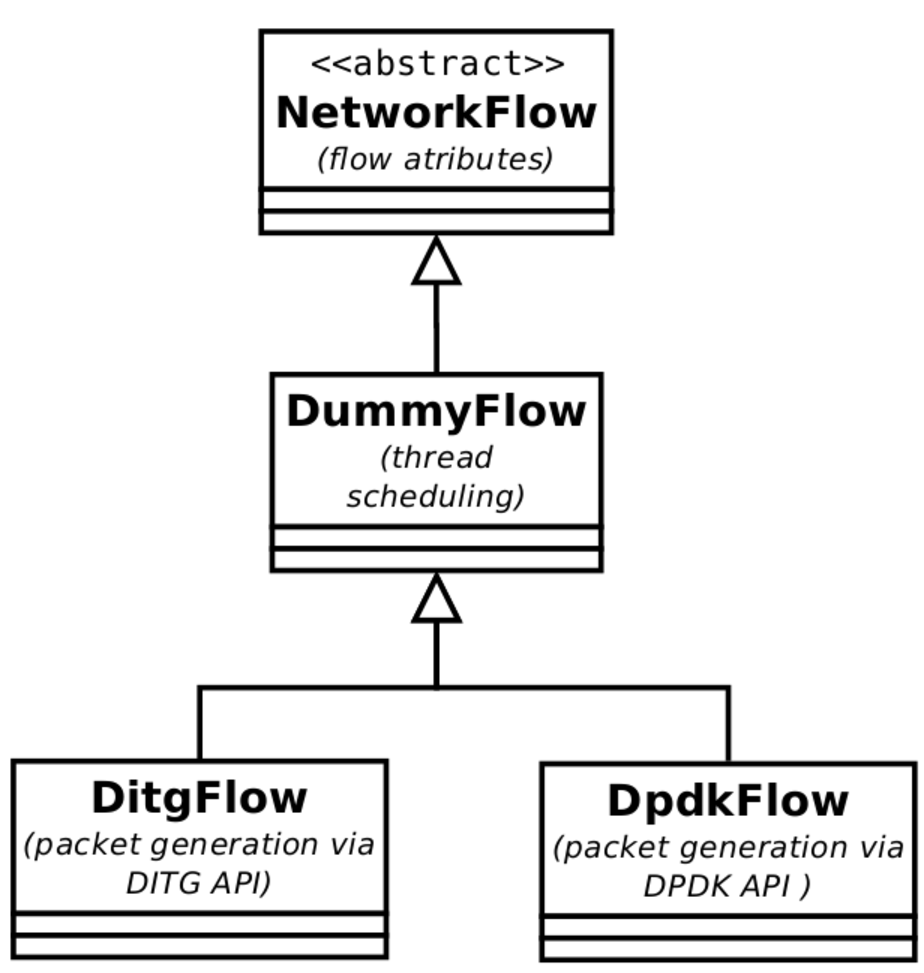
\includegraphics[height=2.0in]{figures/ch6/dpdk-flow}
		\label{fig:dpdk-flow}
	}
	\hspace{0mm}
	\subfloat[DpdkInterface]{
		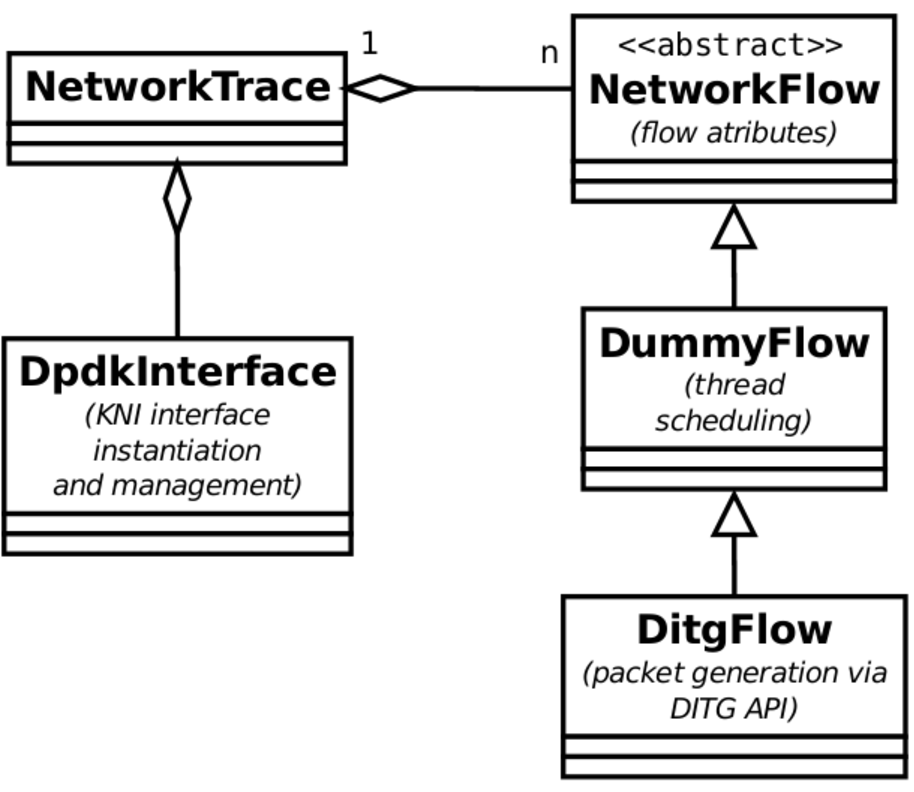
\includegraphics[height=2.0in]{figures/ch6/dpdk-interface}
		\label{fig:dpdk-if}
	}
	\caption{Class diagram for DPDK support expansions. On (a), we have a implementation of traffic generation based on DPDK. On (b) we are using DPDK KNI interfaces.}
	\label{fig:DpdkFlow}
\end{figure}

(6) Another issue is the sniffer component is taking to much time to extract data from large \textit{pcap} files. Implementing a C/C++ multi-thread sniffer, including the packet processing and the SQL queries, will improve its performance. 


(7) SIMITAR's current implementation using \textit{libtins} to generate the packets does not model inter-packet times. To avoid overheads on random numbers calculation,  these values must be calculated before the actual traffic generation. Modelling inter-packet times the scaling characteristics of libtins traffic should improve. 


(8-10) Expand SIMITAR to other traffic generator tools, as we present in the figure ~\ref{fig:DpdkFlow}. D-ITG offers many stochastic functions for customization of inter-packet times, Ostinato provides a rich set of headers and protocols, and DPDK a high performance on packet generation. Each tool can offer a different result on traffic generation, each with benefits and drawbacks, such as computational cost, and development complexity.  Also, DPDK provides the possibility to bypass the Linux network stack, called packet acceleration. So, this implementation can enable for SIMITAR high-bandwidth along with traffic realism.


(11) Calibrate  the constant  \texttt{DataProcessor::min\_time}: smallest time considered for inter-packet times. We use this value to avoid inter-packet times equals to zero due to the sniffer resolution. A zero-inter-packet time would make the procedure fail.  This value can change the fitting accuracy. Today, this value is $5e-8$.


(12) Calibrate  the constant \texttt{DataProcessor::m\_min\_on\_time}: this value controls the small ON time that a \textit{file} can have. It can change the generated traffic precision. Currently this value is $0.1$s. 


(13) Calibrate  the constant \texttt{DataProcessor::m\_session\_cut\_time}: this value defines whatever a file transference still active or has ended. It defines the smallest OFF time acceptable. This value will change how many files SIMITAR will transfer per flow, and how many times it will call the underlying traffic generator. This constant affects the computational performance and traffic realism.


(14) Constant \textit{Control a minimum number of packets required for SIMITAR create a new flow}: this would reduce the number of flows created, improving its computational performance. Since SIMITAR manages each flow in a different thread, it will create fewer threads simultaneously, reducing overheads. This action should not impact on throughput and scaling characteristics because few packets would be ignored. But it can increase the precision of the most significant flows since all the threads are competing for each other on the Operational System. But, the number of flows created would be smaller.


(15) Currently, SIMITAR only enables the programming of flow traffic generation in C++. Adding Python and Lua support for the Flow Generator component, we can enable expansion for Python/Lua traffic generation APIs (such as Ostinato and MoonGen APIs), without creating C++ wrappers.


(16) \textbf{PcapGen: a compact \textit{pcap} lybrary}: Create a component capable of generate synthetic \textit{pcap} files, using Compact Trace Descriptors(CTDs) files. We can implement this using SIMITAR as a packet injector, but in an emulated host interface, for example, using Mininet. Then, the traffic can be collected, using a tool such as TCPDump or Tshark. We present a diagram of this idea in the figure ~\ref{fig:pcap-gen}. This expansion would enable SIMITAR  to work as trace library for pcap-based benchmark tools.


\begin{figure}[!ht]
	\centering
	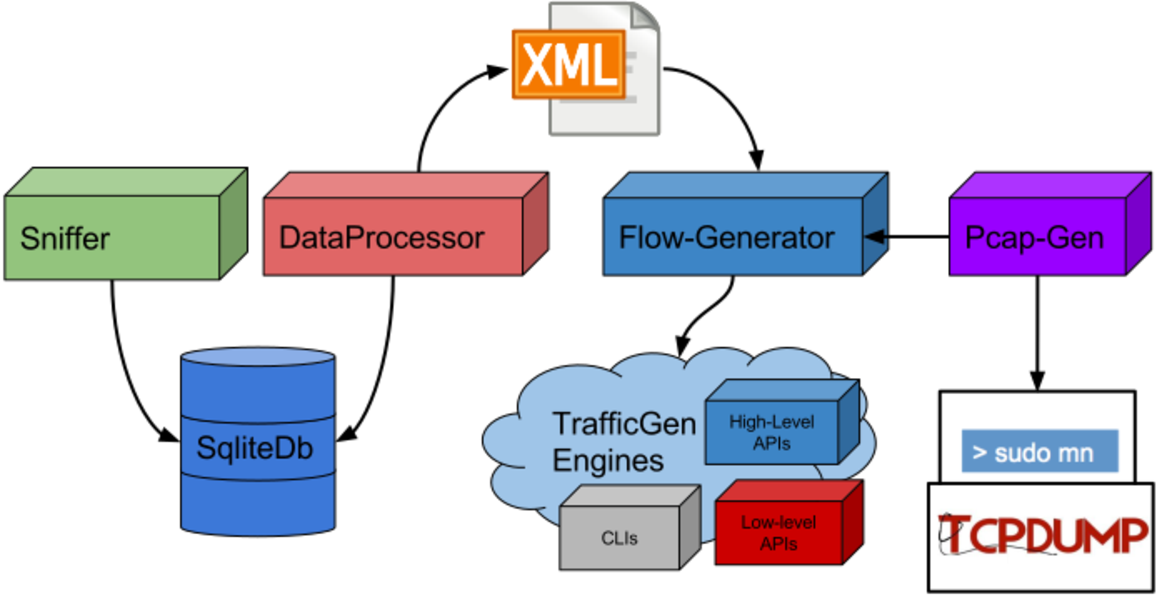
\includegraphics[height=2.0in]{figures/ch6/pcap-gen}
	\caption{Using SIMITAR for generation synthetic \textit{pcap} files, CTD files: a component schema}
	\label{fig:pcap-gen}
\end{figure}
	


%\item \textbf{Use OpenDayLight REST API for data collection}: Another different approach for data collection could be the use the OpenDayLight REST API to collect data from an SDN OpenFlow switches, instead of a using a Sniffer. Through REST API is possible to extract many statistics from nodes, hosts, and ports, such active flows, the number of packets matched per flows, packet drops, and so on. But, different features would be measured,  and a new model for traffic generation would be needed. On the other hand, we could reuse many procedures implemented.  

%\subsection{Changing the Model, reusing the Architecture}

%Since the proposed architecture is model-independent, another future work is to use the same general concepts of compact trace descriptor and API agnostic modeling on different models and compare the results.

%Our proposed future work is to implement this idea using the Swing\cite{swing-paper} and the Harpoon Model\cite{harpoon-paper}.  We can create not just Simitar trace descriptors, but Swing and Harpoon trace descriptors as well. So, as here, we would have the same components: the Sniffer, the SQLite database, the DataProcessor, the flow generator, and the same interface based on an XML Compact Trace Descriptor. The FlowGenerator would abstract the traffic generation in based on the Swing and Harpoon model, in an API independent way as well. 

%These implementations can lead to a definitive and standardized model of realistic traffic generation. In this way, progresses on high-speed traffic generation would no more make old traffic generators and models obsolete. Also, would enable the comparison (ain a fair way) which model is actually the best since the same engine and technic for generating packets will be used.

%Also, the idea of a Compact Trace Descriptor, by itself separates the idea of traffic generation and the modeling. De development of new methodologies for modeling is  separated from the traffic generation. So a data-developer, using any compact trace descriptor interface may just "plug" his method of data modeling in the FlowGenerator. He has not to care about how the packets were going to be generated anymore nor in what programming language is being used to craft packets.


\section{Final Conclusions}


In this dissertation we discuss our process of conceiving, researching, definition and development and validation of an realistic traffic generator able to at the same time fulfill gaps others proposals haven't, and achieve results comparable to the available proposals. This was not a linear procedure. Was indeed an espiral procedure, as proposed by Sommervile on Software Engineering\cite{sommerville}. Clealy its not identical, because we adapt it for research purposes. At the figure~\ref{fig:spiral} we show a diagram of who  it was done. 

\begin{figure}[!ht]
	\centering
	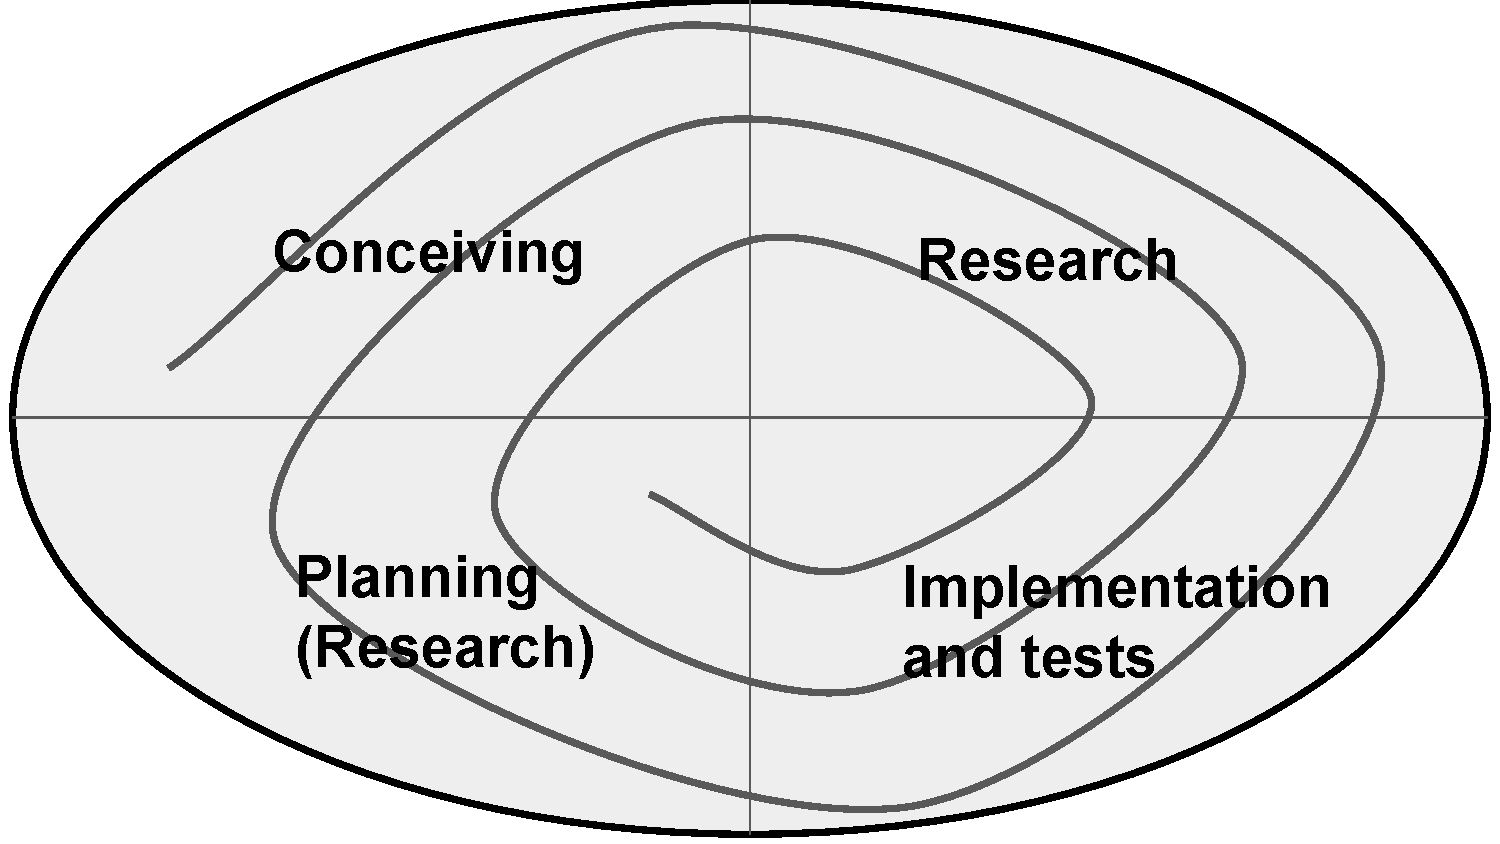
\includegraphics[scale=0.4]{figures/ch6/spiral}
	\caption{Spiral research and development procedure}
	\label{fig:spiral}
\end{figure}


We started defining our goals creating a task list, formalizing it on "Working Plan" documents. These tasks lists covered the whole process and included research, the study of new subjects, implementation, and testing. Next, search on the literature the state of things, related works and points for innovation. At this point, we defined the concepts of our traffic generator. We create an architecture model using UML, defining the software components, classes and sequence diagrams. This initial step was crucial since, in later stages, changes in the architecture design are much more difficult. In fact, some small changes such as directory structure and new classes are inevitable. But structural changes are impracticable. At this point we implemented a simplistic prototype, and validate it\footnote{In the appendix ~\ref{ap:publications}, this prototype is validated in the article "Towards a Flexible and Extensible Framework for Realistic Traffic Generation on Emerging Networking Scenarios"}. 


After this, we search for more solutions and methodologies that could be applied to solve our problems and improve the performance of our prototype. In this procedure, we researched many topics that at the end didn't fit our intentions, such as Machine Learning and Neural Networks. But others such as Linear regression, maximum likelihood, and information criterions (BIC/AIC) were indeed satisfactory. Again, we planned a methodology, procedure, and validate these ideas, as prototypes. Here the seed for the first part of the chapter ~\ref{ch:modeling-evaluation} and the article "Using BIC and AIC for Ethernet traffic model selection. Is it worth?" (in the appendix ~\ref{ap:publications}). Then we research for more related works to gain insights and find platforms and libraries able to fulfill our requirements. In this step, we designed our algorithms presented in chapter ~\ref{ch:modeling-evaluation}, and chose the APIs, packages, and libraries, such as Armadillo\cite{armadillo}, a C++ linear algebra library. Many ideas we used to conceive our ideas were inspired by previous works and solutions, such as Harpoon\cite{harpoon-validation}, sourcesOnoff \cite{sourcesonoff-paper} and LegoTG\cite{legotg-paper}. This procedure continued with incremental upgrades until we arrived on the version presented on the chapter ~\ref{ch:validation}. 


In the chapter ~\ref{ch:modeling-evaluation} we achieve a significant contribution of our work, which shows that the information criteria AIC and BIC are efficient analytical methods for select models for inter-packet times. Both can infer a good model, even evaluated according to different types of metrics, without any simulation. Also, we show evidence that for Ethernet traffic of data, choosing AIC and BIC make almost no difference. As far as is our knowledge, this is a complete study on the use of AIC and BIC on inter-packet times modeling of Ethernet traffic.


In the end, we were able to implement a functional implementation of the solution proposed in the chapter ~\ref{ch:introduction}. Our main contribution here is the development of a traffic generator tool that at the same time can provide realistic synthetic traffic, and its modeling framework is extensible for most of the traffic generation libraries and tools. In fact, our current implementations use tow very distinct packet-crafters: \textit{libtins}, a C++ library designed for the implementation of sniffers and traffic generators, and Iperf, a traffic generator commonly used to measure bandwidth. 


Out tests performed on the chapter ~\ref{ch:validation} intend to focus on packet-level, flow-level and scaling metrics, as we state on chapter ~\ref{ch:literature-review}. The results were notably good at the flow-level. SIMITAR were able to replicate the flow-cumulative distribution with high accuracy, and with \textit{libtins}, the number of flows as well. The number of flows was larger because it establishes additional connections for signaling and statistics control. On scaling and packet matrics, the results still have to be improved. Iperf as the traffic generator tool, still being limited, has proved to be efficient on replication the scaling characteristics for the Skype traffic. Since it establishes socket connections to generate the traffic, we believe that this fact makes it accurate on replication traffic from applications. 


Finally, we created a list of improvements and future works, aiming the improvement of performance on processing time, and packet generation; and the methods to improve the realism of the traffic generated. In the is we believe to overcome the current limitations.





